% ============================
% ME 793 – Computational Fluid Dynamics
% Project 3 Report Template
% REVTeX 4.2e (revtex4-2) + AAPM class
% ============================
\documentclass[
  aapm,
  amsmath,amssymb,
  reprint,          % two-column journal-like layout
  %preprint,        % uncomment for single-column draft
  floatfix
]{revtex4-2}

% ----------------------------
% Packages
% ----------------------------
\usepackage{graphicx}       % figures
\usepackage{dcolumn}        % decimal-aligned table columns
\usepackage{bm}             % bold math symbols
\usepackage{siunitx}        % SI units (optional, but useful)
\usepackage{hyperref}       % clickable references/links
\usepackage{algorithm2e}    % pseudocode (optional)
\usepackage{tabularx}

% ----------------------------
% Title block
% ----------------------------
\begin{document}

\title{Project 3: Flow Around an Actuator Disk Model for UAV Wind Sensor Placement}

\author{Jaden Mecham}
\email{jadenmecham@unr.edu}
\affiliation{Department of Mechanical Engineering, University of Nevada, Reno}

\date{\today}

\begin{abstract}
Accurate wind sensing is critical for UAV flight stability and environmental monitoring, 
but propeller-induced flow can corrupt onboard measurements. This project simulates 
the 2D incompressible flow generated by a hovering rotor using an actuator-disk model, 
governed by the Navier--Stokes equations with a body force representing the rotor thrust. 
The solver extends a fractional-step method on a staggered grid, incorporating the 
disk force into the momentum predictor step. Validation against Froude--Rankine 
momentum theory will be performed by comparing centerline velocities and integrated 
thrust against theoretical predictions. A parameter study over Reynolds numbers 
from 100 to 1000 will be conducted, along with a sensor-placement analysis to identify 
low-disturbance regions for anemometer placement. The project aims to provide insights 
into optimal sensor locations on UAVs while demonstrating proficiency in CFD techniques 
and AI-assisted code development.
\end{abstract}

\maketitle

\section{Introduction}

\section{Governing Equations}
The flow is governed by the incompresible Navier--Stokes equations,
\begin{equation}
  \frac{\partial \mathbf{u}}{\partial t}
  + (\mathbf{u}\cdot\nabla)\mathbf{u}
  = -\nabla p + \frac{1}{Re}\,\nabla^{2}\mathbf{u} + \mathbf{f},
  \qquad \nabla\cdot\mathbf{u} = 0,
\end{equation}
where $\mathbf{f}$ is the actuator-disk body force and
$Re = v_{h} D / \nu$ is the Reynolds number formed from the induced velocity
$v_{h} = \sqrt{T/(2\rho A)}$, the disk diameter $D$, and the kinematic viscosity $\nu$.
Here $T$ is the rotor thrust and $A = \pi D^{2}/4$ is the disk area.

The most important distinction between this project and Project 2 is
the addition of the body force term $\mathbf{f}$, which models the momentum injection
from the rotor.  This term will be implemented as a uniform forcing across a single
column of $u$-face cells spanning the disk diameter, effectively creating a thin band of
momentum source in the flow.  The rest of the numerical method, including the pressure
correction and projection steps, remains unchanged from Project~2, allowing us to leverage
the existing solver infrastructure while extending its capabilities to handle the new 
physics.

\section{Numerical Method}
Much like the previous project, the solver uses a fractional-step (projection) 
method on a staggered grid. The key modification is the inclusion of the actuator-disk 
body force $\mathbf{f}$. The momentum predictor step is updated to:
\begin{equation}
    \mathbf{u}^{*} = \mathbf{u}^{n}
    + \Delta t\!\left[-A(\mathbf{u}^{n})
      + \frac{1}{Re}\,L\,\mathbf{u}^{n} + \mathbf{f}\right],
\end{equation}
where $A$ is the discrete advection operator and $L$ is the vector Laplacian. 
The body force $\mathbf{f}$ is applied uniformly across the disk region, which is
defined as a single column of $u$-face cells that span the rotor diameter. This approach 
allows for a straightforward implementation of the actuator-disk model within the 
existing sparse-matrix framework of the solver.

This project uses the same grid discretization scheme as project 2, with second-order 
central differences on a uniform Cartesian grid. The grid is shown in Figure~\ref{fig:grid}, 
where the $u$-velocity components are stored at the faces of the cells, and 
the $v$-velocity components are stored at the centers of the cells. 
The pressure is also stored at the cell centers. Time integration is performed using 
an explicit Euler method, with a CFL condition of $CFL \leq 0.5$ to ensure stability. 
The pressure Poisson equation is solved at each time step using a conjugate gradient \
solver from the scipy library.

\begin{figure}[h]
  \centering
  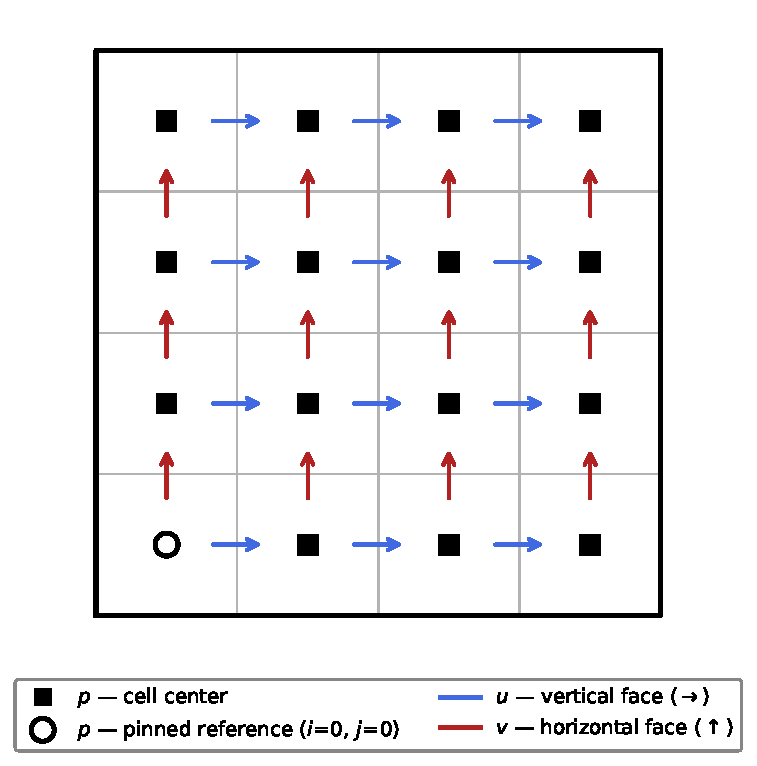
\includegraphics[width=0.85\linewidth]{figs/staggered_grid.pdf}
  \caption{Staggered grid formulation. Horizontal velocity $u$ ({\large$\rightarrow$}),
    vertical velocity $v$ ({\large$\uparrow$}), and pressure $p$ (\ensuremath{\blacksquare})
    are located at cell faces and cell centers, respectively. The open circle ({\large$\circ$})
    marks the pinned pressure reference.}
  \label{fig:grid}
\end{figure}

\section{Verification and Validation}
The primary benchmark for validation is the Froude--Rankine actuator-disk momentum theory, 
which provides analytical predictions for the flow field generated by a hovering rotor. 
According to this theory, the streamwise velocity at the disk plane should equal the 
hover-induced velocity $v_{h}$, and the far-wake velocity should approach $2v_{h}$.

The validation plan includes the following steps:
\begin{itemize}
    \item Compare the centerline velocity one diameter downstream of the disk against the theoretical value of $2v_{h}$.
    \item Compare the integrated thrust extracted from the momentum flux against the prescribed forcing to ensure that the body force implementation is correct.
    \item Compare the radial velocity profile in the far wake against the top-hat actuator-disk prediction to verify that the flow field is being accurately captured.
\end{itemize}

Furthermore, an important conceptual validation step is to ensure that the wind experience
for sensors placed at various locations around the disk matches the expected flow 
disturbance patterns, which will be analyzed in the sensor-placement study. Sensors placed 
in regions of high flow disturbance should experience significant deviations from the 
free-stream velocity, while those in low-disturbance regions should measure velocities 
closer to the ambient conditions. 

\section{Results and Discussion}

\subsection{Free Flow Validation}
The first set of results will focus on validating the wind sensor experience when the 
actuator disk is not present, effectively simulating free flow conditions. This will 
serve as a baseline to ensure that the solver correctly captures the ambient flow field 
without any disturbances from the rotor. The velocity profiles and sensor readings 
in this scenario should match the expected free-stream conditions, providing confidence 
in the solver's ability to accurately model the flow.

\subsection{Ambient Flow Validation}
Next, the results will include the validation of the sensor experience when there is
ambient wind present, but the actuator disk is still not active. This is done just to verify
that the sensors are correctly capturing the ambient flow conditions before
introducing the complexities of the rotor-induced flow. The sensor readings in this case
should reflect the ambient wind velocity and direction, confirming that the sensors are
functioning correctly and that the solver is accurately modeling the ambient flow field.

\section{AI Usage Log}

\section{Conclusions}

\section{Problem Description}

In multirotor drone design, accurate wind sensing is essential for flight stabilization
and environmental monitoring, but propeller-induced flow can corrupt measurements
from onboard wind sensors.  The present study simulates the two-dimensional incompressible
flow generated by a hovering rotor using an actuator-disk model. The propeller is modeled
by a thin band of body force that injects momentum into the fluid.
The flow is governed by the incompressible Navier--Stokes equations,
\begin{equation}
  \frac{\partial \mathbf{u}}{\partial t}
  + (\mathbf{u}\cdot\nabla)\mathbf{u}
  = -\nabla p + \frac{1}{Re}\,\nabla^{2}\mathbf{u} + \mathbf{f},
  \qquad \nabla\cdot\mathbf{u} = 0,
\end{equation}
where $\mathbf{f}$ is the actuator-disk body force and
$Re = v_{h} D / \nu$ is the Reynolds number formed from the induced velocity
$v_{h} = \sqrt{T/(2\rho A)}$, the disk diameter $D$, and the kinematic viscosity $\nu$.
Here $T$ is the rotor thrust and $A = \pi D^{2}/4$ is the disk area.
Target Reynolds numbers of $Re \in [100,\,1000]$ will be explored.

\section{Numerical Approach}

The solver extends the fractional-step (projection) method developed in Project~2
on a staggered grid.  The only structural modification is the addition of the
actuator-disk body force $\mathbf{f}$ to the momentum predictor step:
\begin{equation}
  \mathbf{u}^{*} = \mathbf{u}^{n}
    + \Delta t\!\left[-A(\mathbf{u}^{n})
      + \frac{1}{Re}\,L\,\mathbf{u}^{n} + \mathbf{f}\right],
\end{equation}
where $A$ is the discrete advection operator and $L$ is the vector Laplacian.
The disk force is applied uniformly over a single column of $u$-face cells spanning
the rotor diameter, yielding a spatially compact forcing that is straightforward to
implement within the existing sparse-matrix framework.  The pressure correction step
and divergence-free projection remain identical to Project~2.
Second-order central differences are used on a uniform Cartesian grid with explicit
Euler time integration ($CFL \leq 0.5$), and a scipy CG solver handles the pressure
Poisson system at each step.

\section{Planned Features and AI Integration}

\textbf{Actuator-disk body force module.}
    Implement a sparse forcing vector that injects a prescribed thrust coefficient
    $C_T = T/(\tfrac{1}{2}\rho v_{h}^{2} A)$ into the $u$-momentum equation across
    the disk region, with AI assistance to verify the index mapping
    from the 2D staggered grid to the flattened 1D system.

\textbf{Wake velocity post-processing pipeline.}
    Build routines to extract centerline velocity profiles, compute thrust from
    integrated momentum flux, and compare against theory, with AI assistance for
    the quadrature and plotting.

\textbf{Grid-convergence and time-step study.}
    Automate a sweep over grid resolutions ($32^{2}$ to $256^{2}$), log the
    $L^{2}$ velocity error relative to the analytical hover solution, and produce
    convergence-rate plots, using AI to scaffold the sweep and curve-fitting.

\textbf{Sensor-placement analysis.}
    Map $|\mathbf{u} - \mathbf{u}_{\infty}|$ across the domain to identify
    regions of low flow disturbance suitable for anemometer placement, with
    AI assistance for contouring and thresholding.


\section{Validation Plan}

The primary benchmark is Froude--Rankine actuator-disk momentum theory, which predicts
that the streamwise velocity at the disk plane equals the hover-induced velocity
$v_{h}$, and that the far-wake velocity approaches $2v_{h}$.
The simulation will be validated by comparing (i) the centerline
velocity one diameter downstream against the theoretical value $2v_{h}$,
(ii) the integrated thrust extracted from the momentum flux against the prescribed
forcing, and (iii) the radial velocity profile in the far wake against the
top-hat actuator-disk prediction.

\section{Expected Outcomes and Timeline}

\begin{itemize}
  \item \textbf{Week 1 (Apr.\ 24 -- May 1):}
    Integrate body force term into Project~2 solver. verify steady hover solution
    for a single test case at $Re = 200$.Quantitative validation against momentum theory. grid- and time-step convergence
    study. confirm second-order spatial accuracy.
  \item \textbf{Week 2 (May 1 -- May 6):}
    Parameter study over $Re \in [100,\,1000]$; sensor-placement post-processing.
    generate all figures. Draft final report. compile AI Usage Log. Submit.
\end{itemize}


% ============================
% References
% ============================
\bibliographystyle{aapmrev4-2}
\bibliography{references}


\end{document}
